\documentclass[utf8]{beamer}

\usepackage{beamerthemesplit}
\usepackage{textcomp}
\usetheme[pageofpages=de,% String used between the current page and the
% total page count.
bullet=circle,% Use circles instead of squares for bullets.
titleline=true,% Show a line below the frame title.
alternativetitlepage=true,% Use the fancy title page.
%titlepagelogo=logo-polito,% Logo for the first page.
%watermark=cow-glob-bite,% Watermark used in every page.
watermarkheight=100px,% Height of the watermark.
watermarkheightmult=4,% The watermark image is 4 times bigger
% than watermarkheight.
]{Torino}


\title{GrassCMS}
\author{David Francos, Darío Ferrer, Francisco Sanz}
\date{09 de Marzo de 2012}

\begin{document}

\frame{\titlepage}

\section{Introducción}
\begin{frame}
	\frametitle{¿Qué es GrassCMS?}
	\begin{columns}
	\begin{column}{6cm}
		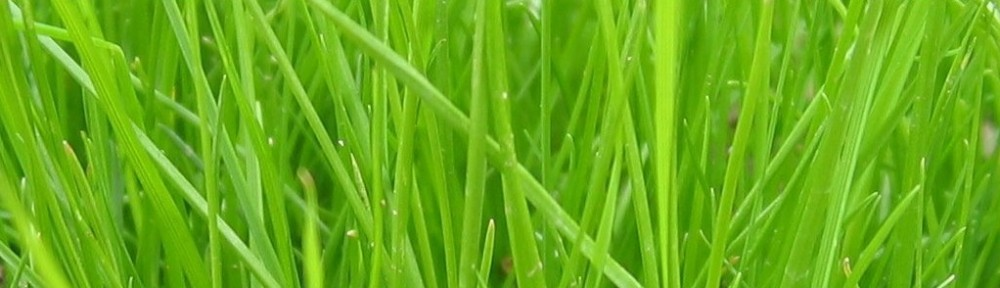
\includegraphics[width=5cm]{images/grass.jpg}
	\end{column}
	\begin{column}{6cm}
		\begin{itemize}
			\item<1->{¿Otro CMS?}
			\item<2->{Grasscms es un proyecto que nace con la idea de dejar en paz al amigo informático}
			\item<3->{El proyecto Grasscms ha reducido la administración web a la mínima expresión}
			\item<4->{Se podría decir que la idea es que las abuelas puedan hacerle la página web a los nietos}
		\end{itemize}
	\end{column}
	\end{columns}
\end{frame}
\section{BOINC}
\begin{frame}
\begin{center}
			
\includegraphics[width=8cm]{images/welcome.png}
\end{center}
\end{frame}

\section{Tecnologías usadas}
\begin{frame}
	\frametitle{Tecnologías usadas}
	\begin{columns}
		\begin{column}{5cm}
			\begin{itemize}
				\item<1->{Flask}
				\item<3->{Flask-gravatar}
				\item<5->{HTML5}
				\item<7->{odt2html.py}
				\item<9->{ckeditor}
			\end{itemize}
		\end{column}
		\begin{column}{5cm}
			\begin{itemize}
			  \item<2->{Flask-openid}
				\item<4->{Twitter Bootstrap}
				\item<6->{Jquery}
				\item<8->{Html5Shiv}
			\end{itemize}
		\end{column}
	\end{columns}
\end{frame}

\section{Características}
\begin{frame}
	\frametitle{Características}
	\begin{columns}
		\begin{column}{5cm}
			\begin{itemize}
				\item<1->{Importación automática odt}
				\item<3->{Subida de ficheros arrastrando desde el escritorio}
				\item<5->{Persistencia}
				\item<7->{Registro vía OpenID}
				\item<9->{Edición simple del perfil}
			\end{itemize}
		\end{column}
		\begin{column}{5cm}
			\begin{itemize}
			  \item<2->{Importación automática txt}
				\item<4->{Drag and drop y cambio de tamaño}
				\item<6->{Generación automática de menús}
				\item<8->{Gravatar}
				\item<10->{Soporte para navegadores antiguos vía \textit{Html5Shiv}}
			\end{itemize}
		\end{column}
	\end{columns}
\end{frame}

\section{Aspecto}
\begin{frame}
	\frametitle{Aspecto}
	\begin{columns}
		\begin{column}{5cm}
			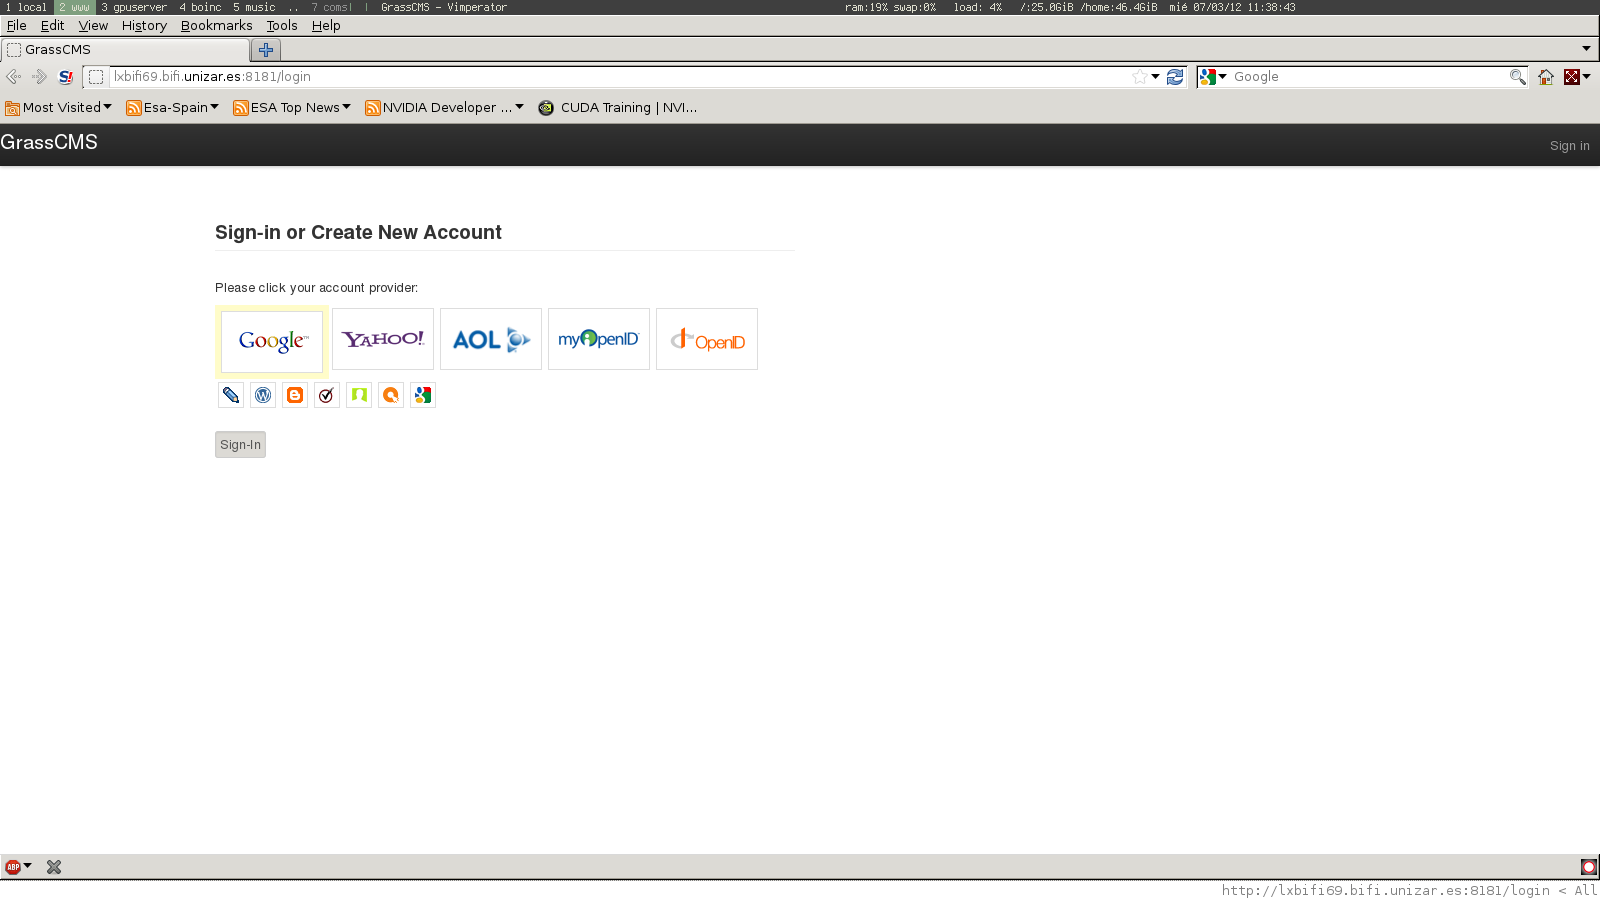
\includegraphics[width=5cm]{images/aspecto1.png}
		\end{column}
		\begin{column}{5cm}
			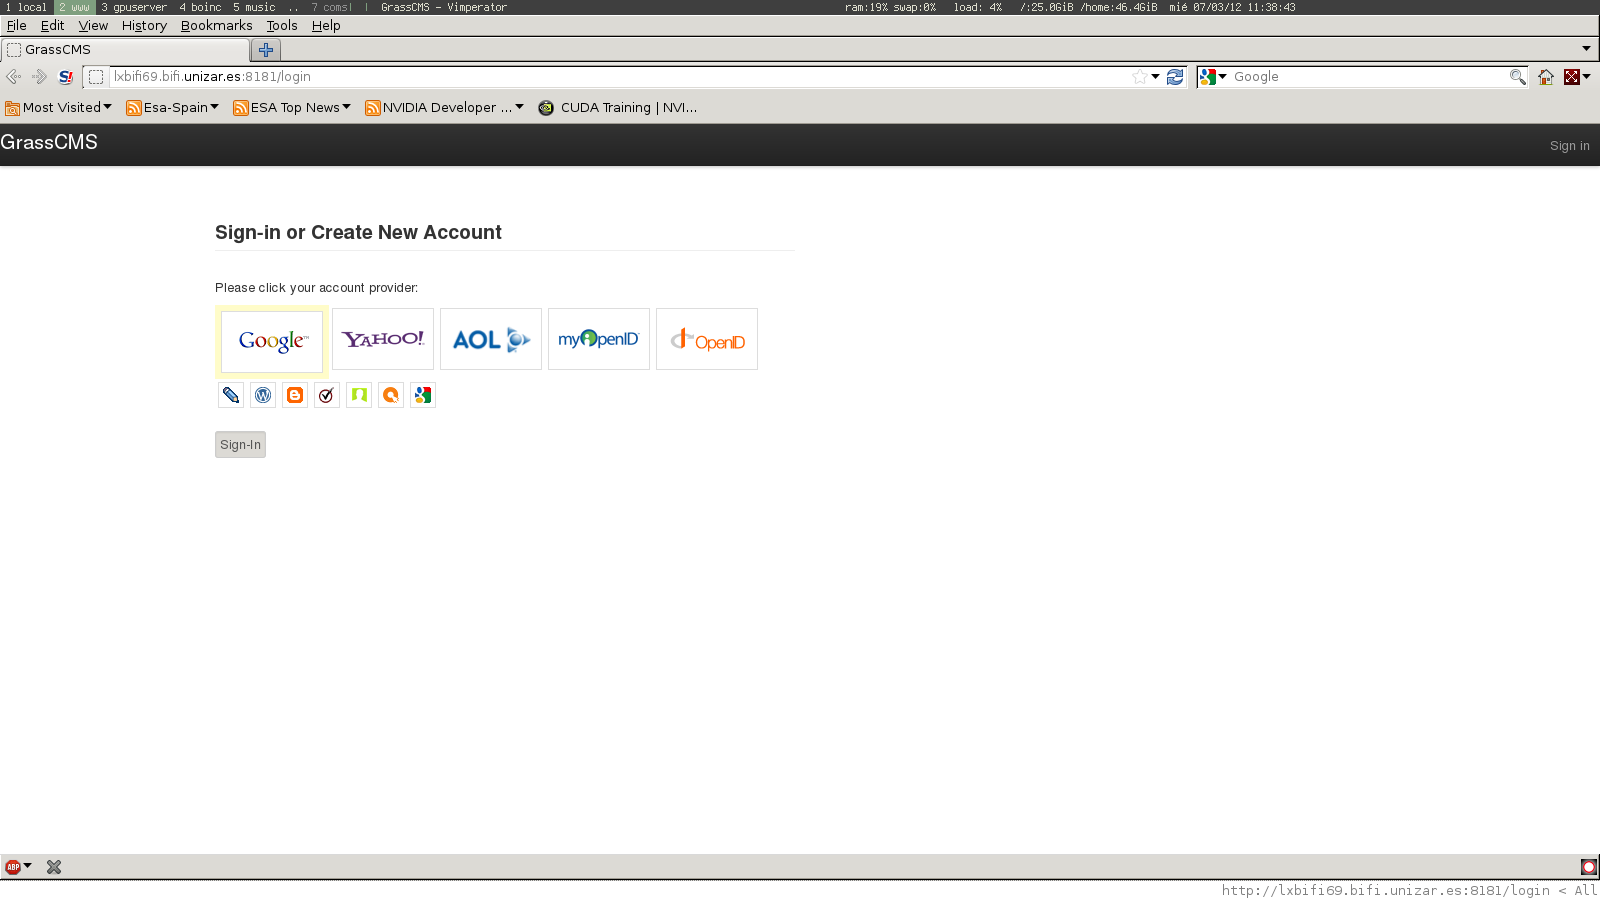
\includegraphics[width=5cm]{images/aspecto1.png}
		\end{column}
	\end{columns}
\end{frame}

\section{Enlaces}
\begin{frame}
	\frametitle{Más información}
	\begin{itemize}
		\item<1->{Hay una compañía detrás de GrassCMS, \textbf{TheOtherNet}}
		\item<2->{\textbf{Blog}: http://www.grasscms.com}
		\item<3->{\textbf{Twitter}: http://twitter.com/grasscms }
		\item<4->{\textbf{Test}: http://test.grasscms.com}
		\item<5->{\textbf{Redmine}: http://acms.traci.es/projects/acms}
		\item<6->{\textbf{SVN en Forja de Rediris}: svn checkout https://forja.rediris.es/svn/cusl6-grasscms}
	\end{itemize}
\end{frame}

\section{Fin}
\begin{frame}
	\frametitle{Fin}
	\begin{center}
		\Huge
		Gracias por vuestra atención
	\end{center}
\end{frame}
\end{document}
